\documentclass[oneside]{book}
\usepackage[a4paper, total={6in, 8in}]{geometry}
\usepackage[italian]{babel}
\usepackage[utf8]{inputenc}
\usepackage{amsmath}
\usepackage{listings}
\usepackage{amssymb}
\usepackage[nottoc]{tocbibind} 
\usepackage{hyperref} 
\usepackage{csquotes}
\usepackage{fancyhdr}
\usepackage{makecell}
\usepackage[font=small,labelfont=bf]{caption} 
\usepackage{pdfpages}
\usepackage{emptypage}
\usepackage{multicol}
\usepackage[ruled,vlined]{algorithm2e}

\pagestyle{fancy}
\fancyhf{}
\lhead{\rightmark}
\cfoot{\leftmark}
\rfoot{\thepage}


\lstset{
    frame=tb, % draw a frame at the top and bottom of the code block
    tabsize=4, % tab space width
    showstringspaces=false, % don't mark spaces in strings
    numbers=left, % display line numbers on the left
    commentstyle=\color{green}, % comment color
    keywordstyle=\color{red}, % keyword color
    stringstyle=\color{blue}, % string color
    breaklines=true,
    postbreak=\mbox{\textcolor{green}{$\hookrightarrow$}\space}
}
  
\date{\textbf{\today}}
\author{
  Giacomo Fantoni \\
  \small Telegram: \href{https://t.me/GiacomoFantoni}{@GiacomoFantoni} \\[3pt]
  Github: \href{https://github.com/whocares/repository}{Github Repository}}

\newcommand{\myparagraph}[1]{\paragraph{#1}\mbox{}\\}
\renewcommand*{\listalgorithmcfname}{}
\renewcommand*{\algorithmcfname}{}
\renewcommand*{\algorithmautorefname}{}
\renewcommand{\thealgocf}{}

\title{\Huge \textbf{Calcolatori}}
\author{
  Giacomo Fantoni \\
  \small Telegram: \href{https://t.me/GiacomoFantoni}{@GiacomoFantoni} \\[3pt]
  \small Github: \href{https://github.com/giacThePhantom/Calcolatori}{https://github.com/giacThePhantom/Calcolatori}}
\begin{document}
\maketitle
\tableofcontents
\chapter{Introduzione}
\section{Tipi di calcolatori}
I calcolatori vengono raggruppati in quattro classi:
\begin{itemize}
\item Personal computer: offrono buone prestazioni per un singolo utente mantenendo il costo limitato. Tipicamente eseguono software di terze parti.
\item Server: calcolatori di dimensioni maggiori orientati verso l'elaborazione di grandi carichi di lavoro come applicazioni scientifiche o per il web.Tipicamente eseguono 
software di terze parti personalizzato. Stesse tecnologie dei personal computer ma con maggiore potenza di calcolo, maggiore velocit\`a di input-output e maggiore capacit\`a di
memoria. Estremamente affidabili.
\item Sistemi embedded: microprocessori progettati per l'esecuzione di applicazioni collegate tra loro implementate con l'hardware. Hanno prestazioni limitate.
\item Dispositivi mobili: si basano su alimentazione a batteria e tecnologie wireless e solitamente i programmi vengono eseguiti in parte su di essi e in parte su appositi 
server dedicati al cloud computing.
\end{itemize}
\section{Esecuzione di un programma}
Il calcolatore \`e in grado di eseguire solamente istruzioni di basso livello semplici e passare da un'applicazione complessa alle semplici istruzioni \`e un processo che \\
coinvolge interpretatori e traduttori che dalle operazioni definite ad alto livello ottengono le istruzioni macchina. Questa gerarchia di operazioni viene divisa in tre 
componenti secondo questa gerarchia:
\begin{enumerate}
\item l'hardware: il calcolatore fisico che esegue le istruzioni.
\item Il sistema operativo che gestisce la base dell'input-ouput, alloca spazio nelle memorie e consente il multi-tasking.
\item Le applicazioni.
\end{enumerate}
\subsection{Da linguaggio ad alto livello a linguaggio macchina}
Per comunicare con una macchina elettronica \`e necessario inviare segnali elettrici (acceso o spento) rappresentati dai numeri $0$ e $1$, che composti formano sequenze di 
numeri binari dei quali ogni cifra \`e detta bit. Un'istruzione \`e pertanto una stringa di bit. Per semplificare il processo di scrittura venne creata una notazione in grado 
di tradurre da un linguaggio di pi\`u facile comprensione a queste stringhe, in questo modo \`e il compilatore stesso a programmare il compilatore. Il primo di questi 
programmi fu chiamato assembler. Se la sequenza di bit viene chiamato linguaggio macchina questa nuova notazione viene chiamata linguaggio assembler. Questa traduzione puntuale
rimaneva ancora di difficile comprensione, vennero creati pertanto linguaggi di programmazione ad alto livello, con particolari compilatori (o interpreti) in grado di tradurrre
questi linguaggi in linguaggio macchina. Questi ultimi pertmettono un incremento di produttivit\`a (condensano pi\`u operazioni) e l'indipendenza dal particolare calcolatore 
sul quale vengono sviluppati. Alcuni compilatori eliminano lo stadio intermedio tra linguaggio di alto livello, assembler e macchina. 
\section{Componenti di un calcolatore}
L'hardware di un calcolatore acquisice dati, li elebora e fornisce il risultato. \`E dotato pertanto di dispositivi di input per la ricezione e di ouptut per l'invio, un'unit
\`a per l'elaborazione dei dati e un'unit\`a di controllo. La parte che esegue le operazioni \`e detta CPU ed \`e formata dalle ultime due parti responsabili per le operazioni
logico-matematiche e per lo spostamento inerno dei dati. La memoria invece \`e il luogo in cui venfono slavati i programmi e i loro dati, costituita da CHIP di DRAM (memoria
dinamica ad accesso casuale). All'interno del processore \`e presente una memoria cache piccola ma veloce che agisce da buffer per la memoria pi\`u grande, costruita di SRAM.
Per permettere l'esecuzione di istruzioni macchina \`e inoltre presente un'interfaccia tra linguaggio di basso livello e hardware: l'architettura dell'insieme di istruzioni, 
checontiene tutte le istruzioni che permettono al calcolatore di funzionare, in modo da evitare al programmatore questo lavoro. Questa architettura \`e indipendente dall'hardware che la implementa, che ne realizza la descrizione. Architettura e sistema operativo costituiscono l'interfaccia binaria delle applicazioni. 
\subsection{Salvare i dati}
La memoria utilizzata per memorizzare i programmi in esecuzione viene detta memoria primaria, \`e volatile e costituita da DRAM. La memoria secondaria, o memoria di massa, 
salva i dati tra un'esecuzione e un'altra, non volatile. Esistono vari tipi di memoria di massa come gli hard disk, o memorie flash a semiconduttore.
\subsection{Comunicazione tra calcolatori}
Il collegamento alla rete ha permesso la condivisione di dati e risorse tra diversi calcolatori attraverso la tecnologia ethernet per le LAN, a fibra per le WAN e wireless per 
i dispositivi portatili. 
\subsection{Produrre un chip}
Un chip \`e formato da transistor su di un circuito integrato prodotto da un wafer di silicio che viene pi\`u volte mascherato, tagliato e "impacchettato". Il costo di un
circuito integrato si pu\`o esprimere con il costo per piastrina: $\frac{\text{Costo per wafer}}{\text{Piatrine per wafer}\cdot\text{Rendimento}}$, le piastrine per wafer:
$\frac{\text{Superficie del wafer}}{\text{SUperfiie della piastrina}}$ e rendimento: $\frac{1}{1+(\text{Difetti per area}\cdot\frac{\text{Area della piastrina}}{2})}$.
\section{Le prestazioni}
Le prestazioni di un calcolatore dipendono da come viene utilizzato: un utente singolo vorr\`a migliorare il tempo di esecuzione, mentre il gestore di un centro di calcolo il
throughput, ovvero il numero di task nell'unit\`a di tempo. In molti casi sono codipendenti. Tenedo conto del tempo di esiscuzione si avr\`a che $Prestaziono=\frac{1}{
\text{Tempo di esecuzione}_X}$. Per controllare quantitativamente le prestazioni di due calcolatori si far\`a il loro prodotto. Le prestazioni di un calcolatore si misurano nel 
tempo totale richiesto ad un calcolatore per completare una task. Siccome i calcolatori lavorano in condizione di condivizione di risorse il sistema potrebbe cercare di 
massimizzare il troughput mettendo in pausa il programma. Si considerer\`a pertanto anche il tempo di CPU, ovvero il tempo effettivamente speso dalla CPU per risolvere il 
programma, che pu\`o essere a sua volta diviso tra tempo di CPU utente (per svolgere il programma) e in quello di sistema necessario per eseguire le funzioni del sistema 
operativo. Per rendere pi\`u facile predirre il tempo di esecuzione di un programma si esprime la velocit\`a con cui il processore esegue le istruzioni e attraverso il ciclo
di clock, un segnale periodico per la sincronizzazione delle funzioni implementate nell'hardware. 
\subsection{Prestazione della CPU}
Il tempo di CPU relativo ad un programma si calcola come il prodotto tra i cicli di clock relativi ad esso e il periodo di clock, o il primo diviso la frequenza di clock.
\subsection{Prestazione delle istruzioni}
Il tempo di esecuzione di un programma dipende dal numero di istruzioni che il calcolatore dovr\`a eseguire. Il tempo di esecuzione totale pu\`o perci\`o venire espresso come
il prodotto tra il numero di istruzioni da eseguire e il tempo medio di esecuzione di ciascuna istruzione. Il numero di cicli di clock per eseguire il programma sar\`a
il numoer di istruzioni del programma per il numero medio di cicli di clock per istruzione (CPI).
\subsection{Misura delle prestazioni}
Si pu\`o pertanto esprimere il tempo di CPU come:
\begin{equation}
\text{Tempo di CPU}=\frac{\text{Numero di istruzioni}\cdot\text{CPI}}{\text{Frequenza di clock}}
\end{equation}
Che evidenziano i tre fattori che influenzano le prestazioni. Essendo che il CPI varia da programma a programma risulta sempre difficile determinare le prestazioni in maniera 
univoca.
\section{La barriera dell'energia}
L'aumento della frequenza di clock e della potenza elettrica assorbita sono aumentate di pari passo fino a che \`e diventato impossibile dissipare il calore generato dalla CPU.
A questo punto si \`e ridotta riducendo la tensione di alimentazione, processo a cui si \`e arrivato ad un limite in quanto diminuendola si aumenta la dispersione di corrente, 
rendendolo pertanto svantaggioso. L'assorbimento di potenza si \`e pertanto rivelato una barriera invalicabile. Essendo infatti la potenza richiesta met\`a del prodotto tra
il carico capacitivo, il quadrato della tensione e la frequenza di commutazione. 
\section{Sisitemi multiprocessore}
Per migliorare le prestazioni si \`e passati a creare microprocessori contenenti pi\`u processori o core. Questo procedimento presenta problemi nel suo utilizzo in quanto ora
\`e necessario bilangiare il carico di lavoro tra tutti i core e ridurre il loro tempo di comunicazione e sincronizzazione. 
\chapter{Le istruzioni MIPS}
Le parole del linguaggio del calcolatore sono dette istruzioni e l'intero vocabolario isieme delle istruzioni, interpretati dall'alto al basso. La semplicit\`a dei dispositivi 
\`e un parametro di grande valore per i caclolatori. Un programma \`e un insieme di istruzioni che viene memorizzato come numeri interpretati dalla macchina come istruzioni.
Le operazioni aritmetiche contengono sempre tre elementi, il primo il luogo in cui viene salvato il risultato e gli altri due i due elementi. Questa descrizione permette di 
mantenere l'hardware semplice. 
\section{Gli operando dell'hardware del calcolatore}
Le istruzioni aritmetiche del MIPS possono essere svolte tra un numero limitato di locazioni particolari: i registri, che rappresentano le primitive utilizzate nella 
prograttazione dell'hardware: i registri. Nei calcolatori della classe dei MIPS sono presenti $32$ registri in quanto minori dimensioni implicano maggiore velocit\`a. Per
questo i tre operandi delle istruzioni aritmetiche devono essere scelti tra i $32$ registri a $32$ bit. Strutture dati pi\`u complesse possono contenere un numero di elementi
maggiore degli elementi presenti nel calcolatore e di conseguenza vengono allocate in memoria. Si rendono pertanto necessari delle istruzioni di trasfermiento che interagiscano
tra la memoria e i registri. Per questo l'istruzione deve contenere l'indirizzo di memoria corrispondente al dato. La memoria pu\`o essere considerata un vettore 
monodimensionale. Attraverso l'istruzione di load viene caricato un valore da memoria a registro. L'indirizzo del dato in memoria vene ottenuto dalla somma della costanto e del
contenuto del secondo registro. L'indirizzo di due parole consecutive differisce di quattro unit\`a. L'operazione complementare, che dal registro salva in memoria si chiama 
store ed ha sintassi simile. I registri richiedono un tempo di accesso minore rispetto alla memoria e pertanto aumentano il throughput. Per evitare l'operazione di load una 
versione delle istruzioni aritmetiche permette di fare un'operazione tra un registro e una costante. L'operazione di spostamento di due registri richiede la somma con la 
costante zero, che per questo viene sempre contenuta nel registro \emph{\$zero}.
\section{Numeri con e senza segno}
I numeri vengono rappresentati in base $2$ con una sequenza di segnali elettrici alti o bassi e il valore della $i$-esima cifra $d$ \`e $d\cdot mBase^i$, dove $i$ assume un 
valore da $0$ e viene incrementato spostandosi verso sinistra. Queste combinazioni di bit sono rappresentazioni di numeri. \`E possibile progettare un circuito logico che svolga
le operazioni aritmetiche con questi numeri, se il risultato di questa operazione supera i bit disponibili avviene un overflow.
\subsection{Numeri con segno}
Una rappresentazione dei numeri con segno \`e data dalla rappresentazione modulo e segno, ovvero un bit, solitamente l'ultimo viene riservato per il segno: 0 se positivo 1 se 
negativo. Presenta degli svantaggi di efficienza e contiene due zeri. Viene pertanto utilizzata la rappresentazione in complemento a 2, ovvero la met\`a dei numeri da $0$ a $2^{31}-1$ utilizza la rappresentazione precedente, mentre da quel numero in poi sono rappresentati i numeri negativi crescenti. Pertanto i numeri positivi presentano degli zeri
iniziali, mentre i negativi degli uni e si ha un solo zero. Il bit di segno, ovvero quello pi\`u significativo, viene moltiplicato per $-2^{31}$. La condizione di overflow si 
verifica quando il bit pi\`u a sinistra non \`e uguale agli infniti bit alla sua sinistra, ovvero quando il bit di segno non \`e corretto. Il bit di segno viene ripetuto fino
a riempire tutti i bit disponibili. Pertanto si utilizza \emph{lb} per caricare un numero con segno e \emph{lbu} per un byte con un numero senza segno. Per invertire il segno
di un numero si invertono tutti i bit e si somma poi 1. Per estendere il segno si riempie a sinistra del valore del bit di segno. Con il complemento a uno non si aggiunge a uno
al numero quando si cambia di segno. 
\section{Le istruzioni nel calcolatore}
Le istruzioni del calcolatore sono memorizzate come una sequenza di segnali che possono pertanto essere rappresentate come numeri. Dato che i registri vengono indirizzati dalle
istruzioni si deve assegnare un numero ad ogni registro. 
\chapter{Aritmetica dei calcolatori}
\section{La codifica}
Una sequenza di zeri e uni viene utilizzata per rappresentare numeri, caratteri, programmi, immagini e suoni. Questi vengono distinti e riconosciuti attraverso una codifica.
\subsection{Codifica dei naturali}
Viene utilizzata la base due per rappresentare i numeri da $0$ a $2^{k-1}$. La sua conversione in base $16$ consiste nel prendere gruppi di quattro bit e trasformarli nella 
cifra corrispondente in base sedici e viceversa. Per convertire da base $10$ si fa la divisione intera e il resto \`e la cifra da porre a sinistra del numero. Per moltiplicare
per una potenza $n$ di due faccio lo shift a sinistra di $n$ cifre. 
\subsection{Codifica degli interi}
Per codificare i numeri negativi possono venire utilizzate le codifiche:
\begin{itemize}
\item Modulo e segno.
\item Complemento a 1.
\item Complemento a 2.
\end{itemize}
\subsubsection{Modulo e segno}
Il bit pi\`u significativo viene utilizzato per codificare il segno $1$ se negativo. Pone dei problemi di efficienza e presenta pi\`u zeri.
\subsubsection{Complemento a 1}
Questa codifica si ottiene invertendo gli zeri con gli uni e viceversa. Contiene comunque due zeri, ma gli algoritmi di somma sono pi\`u veloci: facco la somma bit a bit
e sommo il riporto della cifra pi\`u significativa. Il risultato \`e attendibile se i riporti delle ultime due cifre sono uguali.
\subsubsection{Complemento a 2}
Per ottenere il complemento a due scorro il numero dal bit meno significativo e comincio a invertire il valore dopo aver incontrato il primo $1$, o sommando $1$ al complemento 
a 1. In questo modo si ottiene una codifica unica dello zero. L'overflow si verifica quando l'ultimo bit di segno \`e in disaccordo con il risultato dell'operazione.
\subsection{Codifica dei reali}
\subsubsection{Virgola fissa}
Si pone un punto in cui i bit meno significativi rappresentano la parte decimale. Per cambiare di base la parte decimale moltiplico ricorsivamente per due per quante cifre 
contiene la parte decimale e considero la parte intera. 
\subsubsection{Virgola mobile}
Un numero reale pu\`o essere rappresentato, analogalmente alla notazione scientifica come un numero compreso tra 1 e 2 moltiplicato per un esponente della sua base. Con questa
codifica il bit pi\`u significativo rappresenta il segno, 8 bit sono dedicati all'esponente in complemento a 2 e i restanti dedicati alla mantissa. 
\chapter{Assembly intel}
Si basa su un'architettura CISC
\section{Gestione dei registri}
Per indicare un registro si prepone \%, per un valore immediato \$.Intel posside 16 registri a 64 bit general purpose: \%rax, \%rbx, \%rcx, \%rdx, \%rsi, \%rdi, \%r8, 
\%r9, \%r10, \%r11, \%r12, \%r13, \%r14, \%r15, \%rbp il frame pointer e \%rsp lo stack pointer. Per accedere ai 32 bit meno significativi si sostituisce r con e, per 
accedere ai 16 meno significativi si omette r, di questi 16 per accedere agli 8 pi\`u significatisi si prepone h, ai meno significativi l. Si trovano inoltre due registri 
specializzati: \%rip instrucion pointer (program counter) e \%rflags, ovvero il registro per i flags. 
\section{Convezioni di chiamata}
Il passaggio di parametri di una funzione \`e considerato da 6 registri: \%rsi, \%rdi, \%rcx, \%rdx, \%r8, \%r9, mentre ulteriori argomenti possono essere salvati sullo
stack. I valori di ritorno vengono salvati nei registri \%rax e \%rdx. I registri da preservare sono: \%rbp, \%rbx, \%r12, \%r13, \%r14, \%r15. Esistono due modalit\`a
per richiamare una funzione attraverso l'istruzione call: call address che chiama la subroutine all'indirizzo indicato e call *register che chiama la funzione 
all'indirizzo contenuto nel registro indicato. Il link register viene salvato automaticamente sullo stack, facilitando le funzioni ricorsive. L'istruzione ret preleva
dallo stack l'indirizzo di ritorno da utilizzare nell'instrucion pointer. 
\section{Modalit\`a di indirizzamento}
Esistono varie modalit\`a di indirizzamento in Intel:
\begin{itemize}
\item $<$displacement$>$
\item [$<$displacement$>$]($<$base register$>$)
\item [$<$displacement$>$]($<$index register$>$, [$<$scale$>$])
\item [$<$displacement$>$]($<$index register$>$, $<$base register$>$, [$<$scale$>$])
\end{itemize}
L'indirizzo di memoria corrispondente viene calcolato come $<$displacement$>+<$base$>+<$index$>\cdot<$scale$>$. Dove displacement \`e una costante a 8, 16, 32 o 64 bit, 
index e base sono indirizzi e scale \`e 1, 2, 4 o 8.
\section{Sintassi istruzioni}
Le istruzioni si presentano nella forma $<$opcode$>$[$<$size$>$]$<$source$>$, $<$destination$>$, dove il secondo elemento \`e sia operando che destinazione e deve essere
un registro o un indirizzo di memoria. Il primo pu\`o essere un valore immediato. I due operandi non possono essere contemporaneamente indirizzi in memoria e non \`e
possibile specificare due operandi e una destinazione diversa. $<$size$>$ viene utilizzato per determinare la grandezza degli operandi: b per 8 bit, w per 16, l per 32,  
q per 64. \`E opzionale quando uno dei due operandi \`e un registro, obbligatorio altrimenti. 
\section{Istruzioni frequenti}
A seguire un elenco delle istruzioni aritmetico-logiche più frequenti:
\begin{itemize}
\item mov per scambiare dati fra memoria e registri e viceversa (la destinazione non può essere un valore immediato);
\item push e pop per leggere e salvare dati sullo stack, senza dover modificare lo stack pointer come avviene in MIPS;
\item add (somma) e addc (somma con carry);
\item sub (sottrazione) e subc (sottrazione con carry);
\item mul (moltiplicazione con segno) e imul (moltiplicazione senza segno);
\item div (divisione con segno) e idiv (divisione senza segno);
\item inc (somma 1) e dec (sottrae 1);
\item and, or, xor e not: operazioni logiche bit a bit;
\item lea: load effective address;
\item rcl, rcr, rol, ror: varie forme di rotate;
\item sal, sar, shl, shr: shift aritmetico e logico;
\item jmp: salto incondizionato;
\item je (jump if equal), jnz (jump if not zero), jc (jump if carry), jnc (jump if not carry);
\item neg;
\item cmp: setta i flag facendo una sottrazione, ma senza salvarne il risultato;
\item call e ret: indirizzo di ritorno sullo stack;
\item nop;
\item eventuali istruzioni condizionali.
\end{itemize}
\subsubsection{Load effective address}
Nonoestante questa operazione sia stata implementata per calcolare indirizzi con indirizzamento diverso senza effettuare accessi, risulta utile per effettuare la somma
tra due registri e salvare il risultato in un terzo: lea (\%rax, \%rbx), \%rcx. Nonostante la sintassi sia simile a quella di un indirizzamento non lo si sta 
effettuando.
\subsubsection{Incremento e decremento}
Utilizzate invece di add in quanto permettono di risparimiare 16 bit sull'operazione.  
\chapter{Il processore}
Si descriver\`a la struttura di un processore facendo riferimento a un set di istruzioni ridotto: accesso a memoria, aritmetico logiche e di salto. Le prime due fasi
dell'esecuzione sono comuni a tutte le istruzioni e sono:
\begin{itemize}
\item Prelievo dell'istruzione da memoria.
\item Lettura del valore di uno o pi\`u registri operandi estratti direttamente dai campi dell'istruzione. 
\end{itemize}
Gli altri passi sono simili: tutte le istruzioni a parte quella di jump incondizionato utilizzano la ALU dopo aver letto gli operandi, o per calcolare l'indirizzo nel
caso di istruzioni di accesso a memoria, il calcolo del risultato nel caso di operazioni logico-aritmetiche o per il calcolo del confronto nel caso delle operazioni di 
salto condizionato. Dopo l'utilizzo dell'ALU le operazioni si differenziano: le istruzioni di accesso a memoria richiedono o salvano il dato in memoria, le operazioni
logico aritmetiche salvano il risultato nel registro target, le operazioni di salto condizionato cambiano il valore del program counter. 
\begin{figure}
  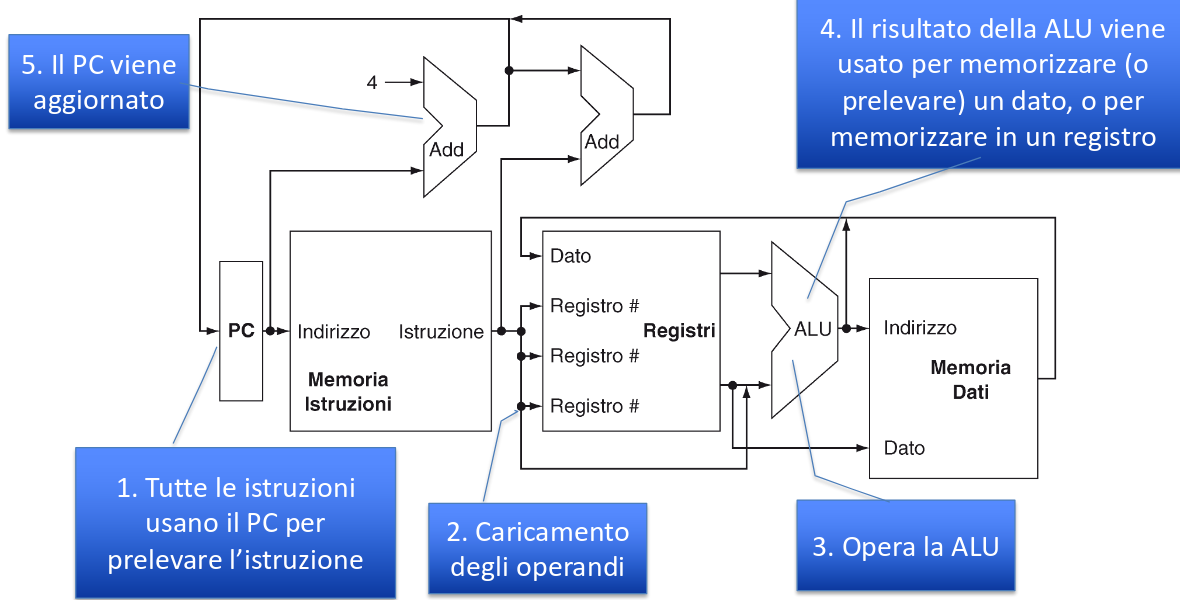
\includegraphics[scale=0.2]{Pictures/CPUBase.png}
  \caption{Un processore base}
  \label{fig:boat1}
\end{figure}
\newpage
La figura precedente \`e incompleta in quanto i dati arrivano da diverse sorgenti dalle quali bisogna scegliere, come per esempio per l'incremento del PC o la differenza
tra istruzioni di tipo R o di tipo I, in cui un dato pu\`o provenire da un registro o essere contenuto nell'istruzione. Per selezionare quale delle operazioni svolgere
viene utilizzato un multiplexer, che sulla base di un ingresso di controllo sceglie quale degli input debba finire in un output. Le linee di controllo del multiplexer 
vengono impostate sulla base del tipo di istruzioni. I vari gruppi funzionali hanno ulteriori ingressi di controllo: la ALU per decidere quale operazione effettuare, il
banco registri ha un ingresso per decidere se scrivere in un ingresso o meno, la memoria dati ha degli ingressi per decidere se si vuole svolgere un'operazione di lettura
o scrittura. La decisione dell'impiego degli ingressi di controllo \`e associata ad un'ulteriore unit\`a funzionale.
\begin{figure}
  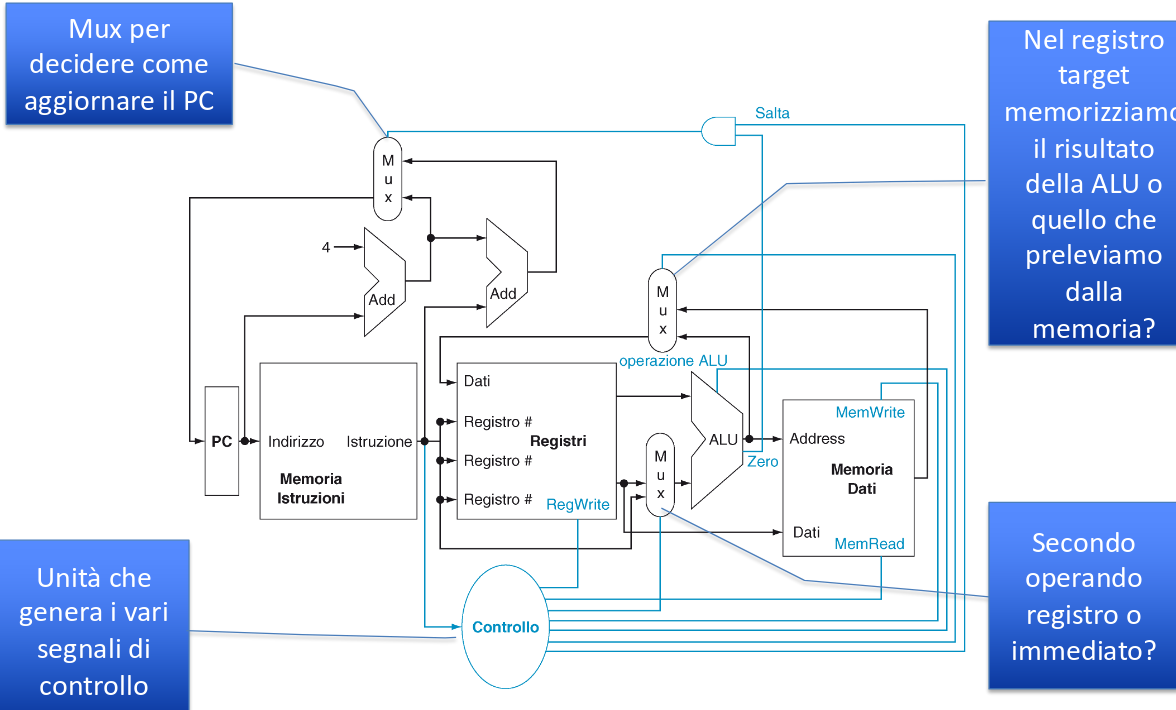
\includegraphics[scale=0.2]{Pictures/CPUDettagliata.png}
  \caption{Un processore pi\`u dettagliato}
  \label{fig:boat1}
\end{figure}
\newpage
Si pu\`o fare un'assunzione semplificativa dicendo che il processore lavora sincronizzandosi con i cicli di clock, e si assuma inoltre che tutte le operazioni si svolgano
in un unico ciclo abbastanza lungo. 
\section{Temporizzazione}
Questa metodologia esplicita quando i segnali possono essere letti o scritti in relazione al clock. Quella pi\`u utilizzata \`e quella sensibile ai fronti, in cui il dato 
viene memorizzato in corrispondenza della salita o della discesa del fronte di clock. I dati presi dagli elementi di stato sono relativi al ciclo precedente. Il tempo 
di clock deve essere scelto in modo da permettere ai dati di attraversare la rete combinatoria. Questa metodologia permette di rendere determinate operazioni che senza
di essa sarebbero indecidibili. 
\section{realizzazione del datapath}
Si passino in rassegna le componenti necessarie per realizzare un datapath:
\begin{itemize}
\item Una memoria istruzioni, dove sono salvate le istruzioni da eseguire.
\item Il program counter, l'indirizzo dell'istruzione da eseguire.
\item Il sommatore, un ALU specializzata a incrementare il PC. 
\end{itemize}
Questi elementi permettono il prelievo dell'istruzione:
\newpage
\begin{figure}
  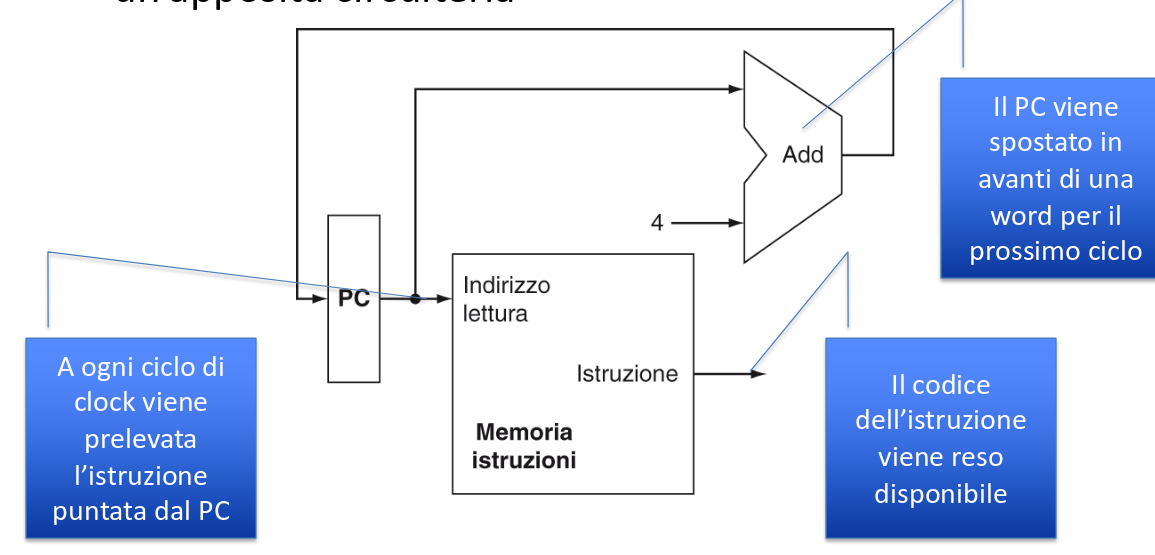
\includegraphics[scale=0.2]{Pictures/PrelievoIstruzione.png}
  \caption{Il processo di prelievo di un'istruzione}
  \label{fig:boat1}
\end{figure}
\subsection{Istruzioni di tipo R}
Le operazioni di tipo R sono istruzioni aritmetico-logiche che operano tra registri e producono un risultato in un altro registro. Per operare queste operazioni si
necessita di altri due blocchi funzionali:
\begin{itemize}
\item Il banco registri, che d\`a in output i registri specificati dell'istruzione e se abilitato in scrittura (regWrite) 0da un multiplexer scrive nel registro 
specificato il dato in ingresso.
\item Una ALU che effettua l'operazione specificata da una codifica a 4 bit, setta un bit in uscita se il risultato \`e zero.
\end{itemize}
\subsection{Istruzioni load store}
Per entrambe si deve calcolare un indirizzo di memoria dato dalla somma di un registro con un offset e nel caso di un'operazione di scrittura leggere il registro dal 
register file. Si necessiter\`a ancora pertanto di ALU e register file. Si noti che essendo l'offset memorizzato in un campo a 16 bit occorrer\`a un'unit\`a funzionale
in grado di estendere il segno a 32 bit. Dovr\`a essere inoltre essere aggiunta un'unit\`a di memoria dati da dove leggere e salvare i dati. Verr\`a utilizzata in 
scrittora (MemWrite) o in lettura (MemRead) in base al segnale dato dall'apposito multiplexer. 
\subsection{Salto condizionato}
Per compiere un salto condizionato si necessita di sommare un offset che dovr\`a essere esteso a 32 bit al PC. Siccome quest ultimo verr\`a sempre automaticamente 
aumentato di 4 verr\`a aggiunto al PC gi\`a aumentato. L'offset inoltre viene automaticamente traslato di due bit in modo da esprimerlo come word e non come byte e 
estendento cos\`i l'intervallo degli offset raggiungibile. Occorre pertanto un ulteriore multiplexer che decida se operare sul PC un'operazione di Pc+4 o PC+4+offset.
Per il salto incondizionato basta sostituire il campo offset shiftato di 4 al PC.
\begin{figure}
  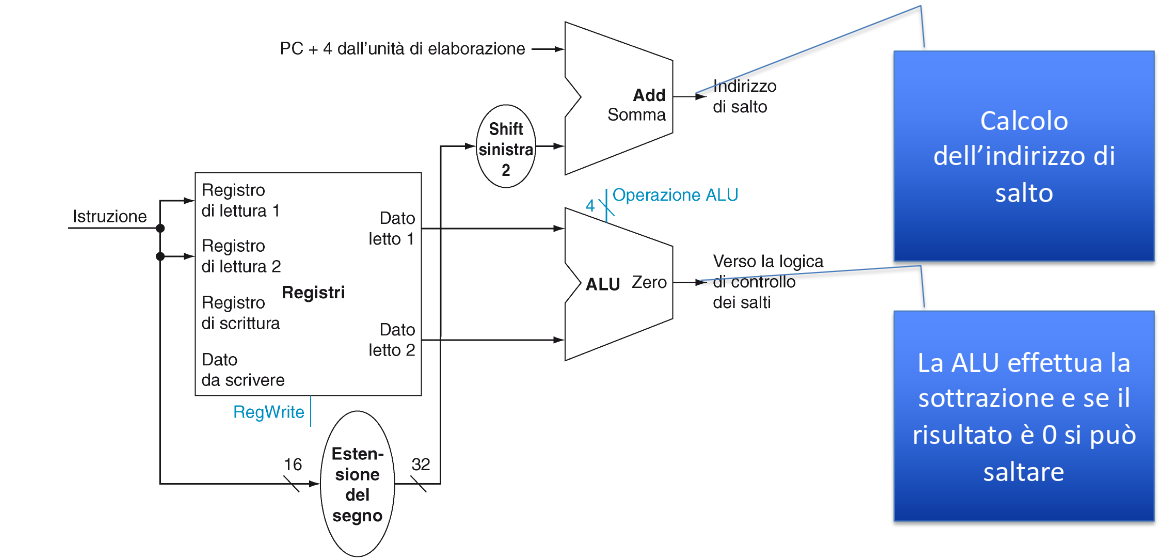
\includegraphics[scale=0.2]{Pictures/SaltoCondizionato.png}
  \caption{Il processo di Salto Condizionato}
  \label{fig:boat1}
\end{figure}
\subsection{Progetto di un'unit\`a di elaborazione}
Siccome ogni unit\`a funzionale pu\`o essere utilizzata un'unica volta per ogni ciclo di clock, si necessiter\`a di distinguere tra memoria dati e memoria istruzioni. 
Occorre inoltre condividere il pi\`u possibile le varie unit\`a. 
\newpage
\begin{figure}
  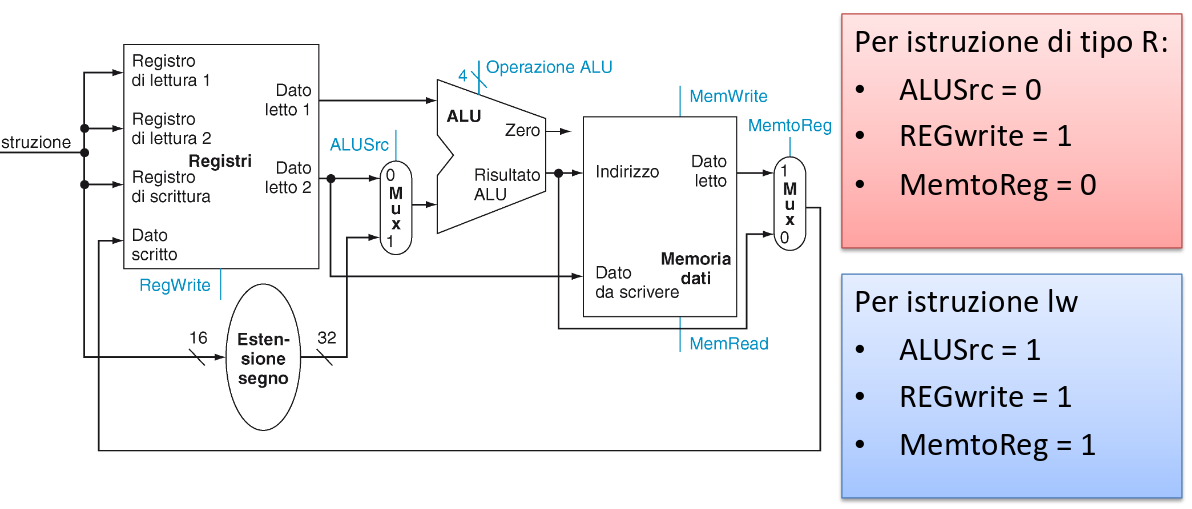
\includegraphics[scale=0.2]{Pictures/RMemoria.png}
  \caption{Circuito per istruzioni R e di trasferimento in memoria}
  \label{fig:boat1}
\end{figure}
\begin{figure}
  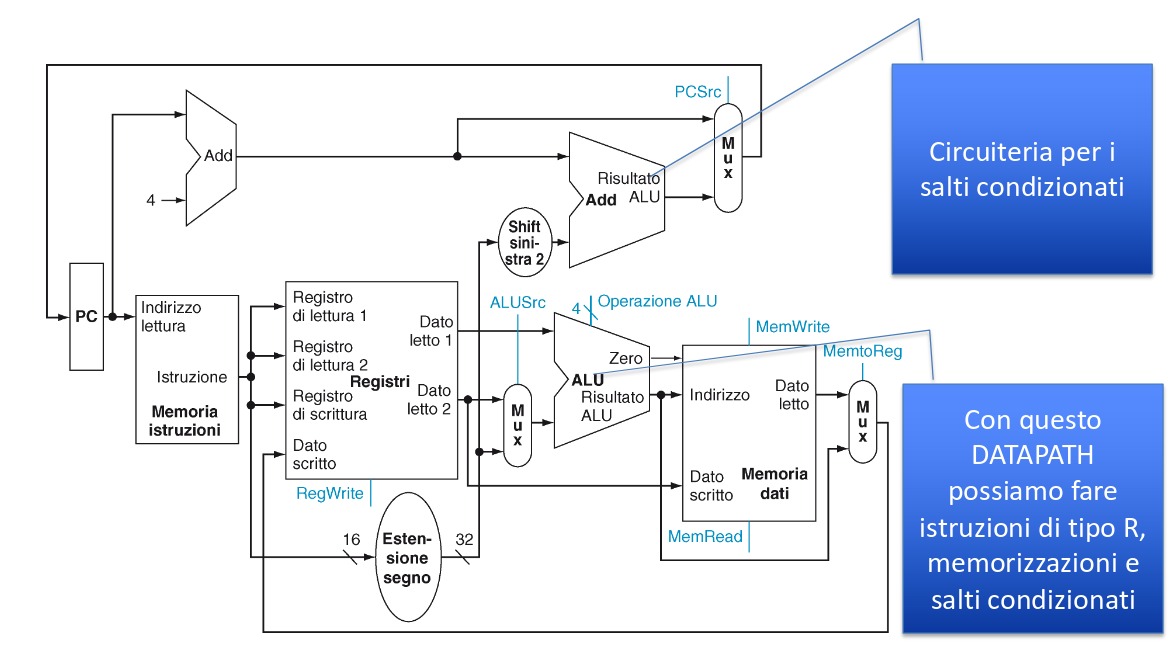
\includegraphics[scale=0.2]{Pictures/RMemoriaCompleto.png}
  \caption{Circuito per istruzioni R e di trasferimento in memoria dettagliato}
  \label{fig:boat1}
\end{figure}
\subsection{Prima implementazione comleta}
Per arrivare a una prima implementazione completa si parta dal datapath mostrato e si aggiunga la parte di controllo, implementando le istruzioni add, sub, and, or, slt, 
lw, sw, beq e successivamente il jump. 
\subsubsection{ALU}
La ALU viene utilizzata per realizzare operazioni logico aritmentiche di tipo R e slt, calcolare indirizzi di memoria e la sottrazione per beq. Per queste operazioni si
ha una diversa configurazione degli input di controllo (a 4 bit), si veda la tabella sulle slide. Per generarli si utilizza un'unit\`a di controllo che prende in 
ingresso il campo funct prelevato dall'istruzuione e due bit detti ALUop, ovvero 00 per sw e lw, 01 per beq, 10 per operazioni di tipo R specificate dal funct. Si genera
pertanto un comando attraverso due livelli: il primo genera i segnali di controllo ALUop per l'unit\`a di controllo della ALU, il secondo genera i segnali di controllo
per la ALU. I segnali di controllo della ALU sono generati da una rete logica combinatoria e per evitare di elencare tutte le combinazioni di ingresso ALUop e dei campi
funct vengono compressi attraverso l'utilizzo della wildcard X. Si vedano le tabelle delle slides.
\newpage
 \begin{figure}
  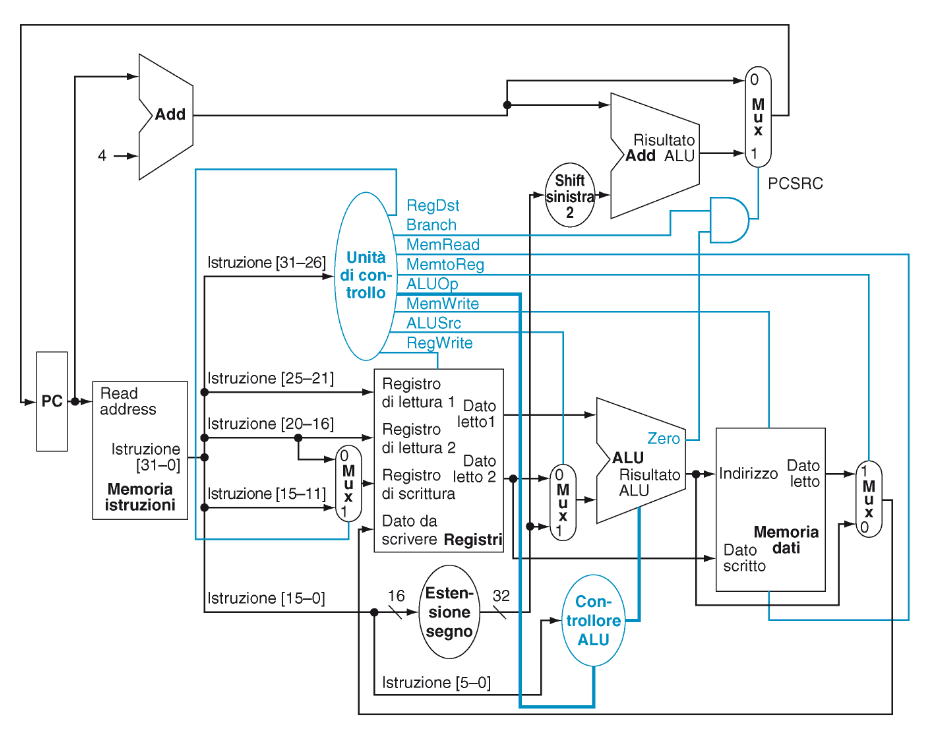
\includegraphics[scale=0.2]{Pictures/CPUComplessiva.png}
  \caption{Una CPU molto dettagliata}
  \label{fig:boat1}
\end{figure}
Si faccia riferimento alle slides per una spiegazione dei segnali di controllo. 
\subsubsection{Unit\`a di controllo}
\`E un'unit\`a funzionale combinatoria che prende come input il codice operativo dell'istruzione e genera i comandi del caso 
\subsubsection{Salto incondizionato}
In questa operazione il PC viene incrementato di 4, i suoi quattro bit significativi rimangono uguali, dal 27 al 2 sostituiti con il campo indirizzo dell'istruzione 
i due bit meno significativi settati a 0.
\section{Conclusione}
Le istruzioni raramente vengono concluse in un unico ciclo in quanto sono le pi\`u lente a dettarlo e non si riesce a fare ottimizzazioni aggressive sulle cose pi\`u 
frequenti.

\chapter{La pipeline}
Si \`e notato come compiere un'operazione per ciclo di clock \`e inefficiente, pertanto si utilizza una pipeline. Si noti come le istruzioni del MIPS hanno 5 fasi 
di esecuzione: prelievo dell'istruzione dalla memoria, lettura dei registri e decodifica dell'istruzione, esecuzione di un'istruzione o calcolo di un indirizzo, accesso
a un operando nella memoria dati, scrittura del risultato in un registro, verr\`a utilizzata pertanto una pipeline a 5 stadi. In una pipeline quando un istruzione termina
l'utilizzo di un elmento funzionale questo viene subito occupato dall'istruzione successiva. 
\subsubsection{Confronto di prestazione}
Il confronto pu\`o essere fatto come tempo fra due istruzioni=$\frac{Tempo\ tra\ due\ istruzioni\ senza\ pipeline}{numero\ stadi\ della\ pipeline}$.
\section{Vantaggi del RISC}
\begin{enumerate}
\item Essendo tutte le istruzioni della stessa lunghezza il prelievo \`e pi\`u facile.
\item Essendo i codici degli operandi in posizione fissa ci si pu\`o accedere leggendo il register file in parallelo con la decodifica dell'istruzione.
\item Gli operandi residienti in memoria sono utilizzabili solo da sw e lw, pertanto si pu\`o utilizzare la ALU per calcolare gli indirizzi. .
\item L'uso di accessi allineati permette agli accessi in memoria di avvenire in un solo ciclo impegnando un solo stadio della pipeline. 
\end{enumerate}
\section{Hazard}
In condizioni normali la pipeline permette di eseguire un'operazione per ciclo di clock, ma ci sono dei casi in cui questo non \`e possibile per il verificarsi di 
condizioni critiche.
\subsection{Hazard strutturali}
L'architettura del calcolatore rende impossibile l'esecuzione di alcune istruzioni in pipeline, ad esempio, disponendo di un'unica memoria non \`e possibile caricare 
istruzioni e prelevare operandi nello stesso ciclo di clok.
\subsection{Hazard sui dati}
Si verifica quando la pipeline deve essere messa in stallo per ottenere informazioni dagli stadi precedenti, come somme che utilizzando gli stessi operandi. Questo 
tipo di hazard blocca la pipeline per tre cicli di clock.
\subsubsection{Possibili soluzioni}
\begin{itemize}
\item In certi casi si pu\`o eliminare il problema a livello di compilatore invertendo delle istruzioni.
\item \`E utile osservare come non \`e necessario salvare il risultato, attraverso un operazione di operand forwarding o propagazione, in cui il risultato viene reso 
disponibile bypassando l'operazione di storage.
\end{itemize}
\subsection{Hazard sul controllo}
Si verifica in presenza di salti condizionati, supponendo di avere un circuito sofisticato che permette di calcolare l'indirizzo di salto si necessita comunque di saltare
uno o due cicli. Se la pipeline \`e troppo lunga questo stallo diventa troppo costoso. Vengono pertanto implementati dei circuiti che prevedano dei salti e fanno delle 
assunzioni su di essi, mettendo le operazioni nella pipeline in base ad esse e poi, se necessario si corregge. Si pu\`o considerare che il salto non venga utilizzato, 
o che il comportamento rimanga costante per esempio. 
\chapter{Le memorie}
La memoria \`e fondamentale per il funzionamento di un compilatore. \`E necessario poterci leggere e scrivere dati. La memoria indirizzata direttamente (memoria 
principale o cache) \`e volatile ed \`e limitata dallo spazio di indirizzamento dal compilatore. Esiste una memoria indirizzata indirettamente o periferica, permanente
con uno spazio di indirizzamento software non limitato dal processore. Le informazioni sulla memoria principale sono disponibili al processore in qualsiasi momento, 
mentre le informazioni nella memoria periferica devono essere prima trasferite a quella principale. Questo trasferimento \`e tipicamente mediato dal sistema operativo.
\begin{itemize}
\item Si intende per tempo di accesso il tempo di un'operazione di lettura o scrittura nella memoria.
\item Il tempo di ciclo \`e il tempo che intercorre tra l'inizio di due operazioni tra locazioni diverse.
\item Accesso casuale: non vi \`e alcuna relazione o ordine tra i dati salvati, tipico delle memorie a semiconduttori.
\item Accesso sequenziale: l'accesso alla memoria \`e ordinato o semi ordinato, il tempo di accesso dipende dalla posizione, tipico dei dischi o dei nastri.
\item RAM (random access memory) memoria scrivibile leggibile a semiconduttori, con tempo di accesso indipendente dalla posizione del dato.
\item ROM (read only memory) memoria a semiconduttori in sola lettura pu\`o avere accesso casuale o sequenziale. 
\end{itemize}
\section{Memorie RAM a semiconduttori}
Queste memorie memorizzano singoli bit spesso organizzati in byte e o word. Data una capacit\`a N la memoria pu\`o essere organizzata in diversi modi a seconda del
parallelismo, influenzando il numero di pin I/O necessari al circuito integrato che la implementa.
\subsection{Memorie statiche SRAM}
Sono memorie in cui i bit possono essere salvati indefinitamente fintanto che rimangono alimentate, sono estremamente veloci e consumano poca corrente, ma sono care
in quanto richiedono molte componenti per ciascuna cella di memorizzazione.
\begin{figure}
  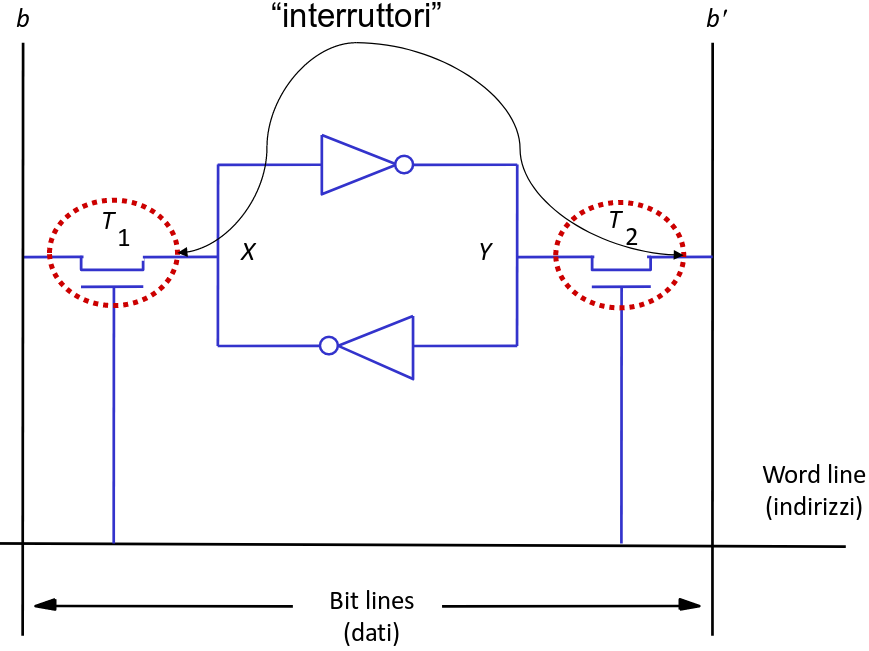
\includegraphics[scale=0.2]{Pictures/SRAM.png}
  \caption{Un bit in SRAM}
  \label{fig:boat1}
\end{figure}
Si consideri che $b=NOT(b')$, i circuiti di terminazione della linea di bit (sense/write circuit) interfacciano il mondo esterno che non accede mai direttamente alle 
celle, la loro presenza contemporanea riduce gli errori. In caso di scrittura la linea di word \`e alta e chiude $T_1$ e $T_2$, il valore presente su b e b', linee di 
pilotaggio viene salvato nel latch a doppio NOT. In caso di lettura la linea di word \`e alta e chiude $T_1$ e $T_2$, il le linee b e b' sono tenute in stato di alta 
impedenza e il valore in X e Y viene copiato in b e b'. Se la linea di word \`e bassa il consumo \`e nullo. 
\subsection{Memorie DRAM}
Sono le memorie pi\`u diffuse in quanto economiche e a densit\`a elevata, in quanto la memoria viene ottenuta sotto forma di carica di un condensatore. Hanno bisogno
per\`o di un costante refresh altrimenti la carica si disperderebbe a causa di correnti parassite.
\begin{figure}
  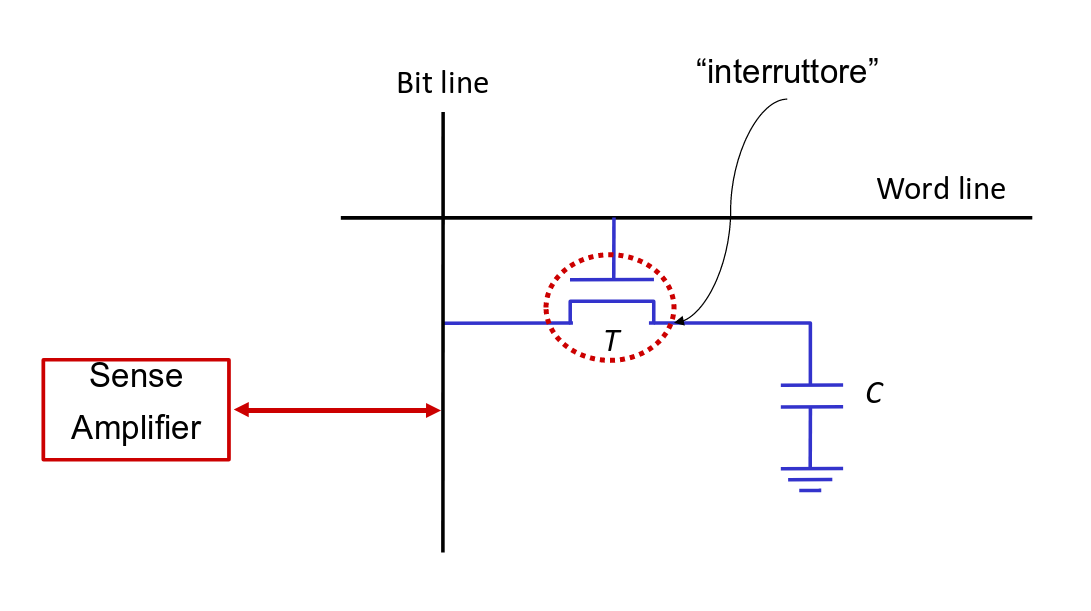
\includegraphics[scale=0.2]{Pictures/DRAM.png}
  \caption{Un bit in DRAM}
  \label{fig:boat1}
\end{figure}
In caso di operazione di scrittura la linea di word \`e alta e chiude T e il valore di b viene copiato su C. In caso di lettura la linea di word chiude T e si utilizza
un apposito circuito che se la tensione di C \`e sopra una certa soglia pilota la linea b alla tensione di alimentazione ricaricando C, altrimenti mette b a terra 
scaricando C.
\subsubsection{Refresh}
Nel momento in cui T \`e aperto il condensatore comincia a caricarsi o scaricarsi a causa di correnti parassite sul semiconduttore e si rende necessario quindi 
periodcamente rinfrescare i dati attraverso un'operazione di lettura. In genere la memoria contiene un circuito per la lettura periodica della memoria, pertanto 
l'utente non se ne deve preoccupare.
\subsubsection{Multiplazione degli indirizzi}
Data l'elevata integrazione delle DRAM il numero di pin I/O diventa un problema, pertanto \`e usuale multiplare nel tempo l'indirizzo delle righe e delle colonne negli
stessi fili. Le memorie non sono indirizzabili al bit, per cui righe e colonne si riferiscono a byte e non a bit. 
\subsubsection{Modo di accesso veloce}
L'accesso ai dati della memoria DRAM avviene da blocchi o pagine di memoria: l'indirizzo viene separato in row address selector e column address selector, il primo dei 
quali estrae una riga dalla pagina e il secondo la colonna dalla riga. \`E possibile, attraverso il fast page mode (FPM) evitare di riselezionare la riga ad ogni accesso
se le posizioni sono consecutive con aumenti delle prestazioni significativi. 
\subsection{Memorie DRAM sincrone SDRAM}
Le DRAM viste prima sono dette asincrone in quanto non esiste una precisa temporizzazione di accesso, ma la dinamica viene governata dai RAS e dai CAS. Il processore
deve tenerne conto in quanto pu\`o generare problemi in fase di refresh. Aggiungendo dei buffer di memorizzazione degli ingressi e delle uscite si pu\`o ottenere 
un funzionamento sincrono disaccoppiando lettura e scrittura dal refresh, ottenendo automaticamente un FPM pilotato dal clock. 
\subsection{Double data rate SDRAM: DDR-SDRAM}
Una SDRAM che consente il trasferimento dei file sia sul fronte positivo che quello negativo del clock. Latenza uguale a una DRAM normale ma banda doppia, le memorie
sono separate in due banchi uno per le locazioni pari sul fronte positivo e l'altro per le locazioni dispari sul fronte negativo. Le locazioni contigue sono in banchi
separati pertanto si pu\`o fare un accesso interlacciato. 
\section{Velocit\`a e prestazione}
\subsubsection{Latenza}
Il tempo di accesso ad una singola parola, d\`a un indicazione al tempo che un processore dovr\`a aspettare un dato dalla memoria nel caso peggiore.
\subsubsection{Velocit\`a o banda}
Indica la velocit\`a di trasferimento massima in FPM, importante per operazioni in FPM che sono legate all'uso di memorie cache interne ai processori. 
\section{Gerarchie di memoria}
Si pu\`o ottimizzare l'utilizzo di memorie in modo da dare l'impressione di avere una grande memoria veloce.
\subsubsection{Localit\`a temporale}
Quando si fa uso di una locazione \`e molto probabile che verr\`a riutilizzata presto.
\subsubsection{Localit\`a spaziale}
Quando si fa riferimento ad una locazione \`e molto probabile che nelle operazioni successive si far\`a riferimento alle locazioni successive.
\subsection{Struttura della gerarchia}
Costi e velocit\`a delle memorie creano una propensione a utilizzare delle piccole e veloci vicino al processore che si ingrandiscono e rallentano allontanandosi da 
esso.
\subsubsection{Terminologia}
\begin{itemize}
\item Si indica con blocco l'unit\`a minima di informazione che pu\`o essere presente o assente in un livello.
\item Hit rate: la frequenza di accesso, la frazione degli accessi in cui trovo il blocco nel livello superiore. 
\item Miss rate: il complementare dell'hit rate.
\item Tempo di hit: il tempo che occorre per trovare il dato quando lo trovo nel livello superiore. 
\item Penalit\`a di miss: il tempo necessario per accedere al dato se non lo trovo nel livello superiore
\end{itemize}
La penalit\`a di miss \`e molto maggiore del tempo di hit e del trasferimento in memoria di un singolo dato, pertanto \`e cruciale che non avvenga troppo spesso. 
\subsection{Cache}
Un posto sicuro, o nascosto dove riporre i dati, nascosto in quanto \`e impossibile accedervi direttamente. Per capire se un dato \`e nella cache o no si pu\`o 
utilizzare una cache a mappatura diretta, ovvero a ogni indirizzo della memoria corrisponde una precisa locazione della cache, l'indirizzo di locazione dove un indirizzo
\`e mappato \`e l'indirizzo del blocco modulo numero di blocchi nella cache. Se il numero di elementi della cache \`e a potenza di due \`e sufficiente prendere i bit 
meno significativi dell'indirizzo in numero pari al logaritmo in base due della potenza della cache. Siccome molte parole possono essere mappate sullo stesso blocco di 
cache per capire se in un dato momento vi si trova l'indirizzo ricercato si ricorre ad un campo, detto tag, che contiene informazione sufficiente a risalire al blocco 
correntemente salvato in memoria, si possono utilizzare per esempio i bit pi\`u significativi di una parola per trovare la locazione in cache dove l'indirizzo \`e 
mappato. Vengono utilizzati i bit pi\`u significativi per capire se nel blocco di cache viene memorizzato l'elemento richiesto, inoltre c'\`e un blocco di validit\`a
che dice se quello che viene memorizzato in un blocco di cache in un dato momento \`e quello richiesto. 
\subsubsection{Prestazioni}
Blocchi di cache molto grande esaltano la localit\`a spaziale e diminuiscono la probabilit\`a di miss. Tuttavia a parit\`a di grandezza della cache blocchi molto grandi 
diminuisce l'efficacia della localit\`a temporale, oltre a generare dei miss con costo elevato. Si necessita pertanto di dover trovare un equilibrio. 
\subsubsection{Gestione delle miss}
La presenza di una cache modifica la gestione della pipeline solo nel caso in cui ci sono delle miss, quando bisogna generare uno stallo nella pipeline per gestire il
trasferimento da memoria principale a cache. Per una miss sulla memoria istruzioni bisogner\`a inviare alla memoria il valora PC-4, eseguire una lettura, scriverne il
risultato aggiornando il tag e far ripartire la fetch. Gli accessi in lettura alla memoria dati avvengono alla stessa maniera.
\subsubsection{Miss in scrittura}
Gli accessi in scrittura sono delicati in quanto possono generare delle inconsistenze. Possono venire implementate due politiche:
\begin{enumerate}
\item Write-through, in cui ogni scrittura viene fatta direttamente in memoria principale, eliminando i problemi di consistenza ma aumentando i costi, si pu\`o impiegare
un buffer di scrittura, una coda con tutte le scritture in attesa di essere completate.
\item Write-back, in cui se il blocco \`e in cache le scritture avvengono localmente in cache e l'update viene fatto solo quando il blocco viene rimpiazzato. Conveniente
in presenza di numerose scritture. 
\end{enumerate}
\subsubsection{Cache completamente associativa}
In questo tipo di cache si pu\`o mappare qualsiasi tipo di blocco in qualsiasi blocco di cache, il loro problema \`e che rendono necesario cercare ovunque il dato, per
essere efficiente su tutti i blocchi in parallelo, si necessitano pertanto n comparatori che operino su n blocchi. Il costo \`e molto elevato, pertanto viene utilizzata 
solo per cache molto piccole. 
\subsubsection{Cache set-associativa}
\`E una via di mezzo tra la mappatura diretta e la completamente associativa: ogni blocco di memoria pu\`o essere mappato su una linea di n blocchi diversi di cache. Si combinano pertanto le due idee: a 
ciascun blocco di memoria viene associata una certa linea, pertanto uno degli n blocchi di quella liena su cui si pu\`o mappare il blocco di memoria e all'interno della linea si effettua una ricerca parallela come
se fosse una cache completamente associativa.  Ovvero un blocco di memoria viene mappato nella linea data da indirizzo blocco modulo numero linee della cache. Pertanto per trovare il blocco all'interno della
linea si deve confrontare in parallelo il tag del blocco con tuti i tag dei blocchi di quella linea.  Aumentando l'associativit\`a diminuisce la frequenza di miss, ma si rendono necessarie operazioni complesse. 
Inoltre nelle cache a mappatura diretta in caso di miss so sicuramente chi sostituire, nelle cache associative si possono utilizzare diverse strategie, come una FIFO o una Least Recently Used.

\chapter{Input-output}
I dispositivi di I/O sono necessari al computer per comunicare con l'esterno, devono essere espandibili ed eterogenei. La tipologia di prestazione varia dai casi: 
nel caso di tastiere e mouse interessa pi\`u la latenza, nel caso di dischi o interfacce di rete interessa pi\`u il throughtput. Questi dispositivi sono collegati al
processore da un dispositivo di comunicazione chiamato bus. I dispositivi i I/O possono essere classificati in base alle operazioni che compiono: read o write, in base
al loro partner (uomo o macchina) e in base alla velocit\`a di trasferimento. 
\section{Connesione tra processori e periferiche}
Le connessioni avvengono tramite delle strutture di comunicazione chiamate bus che si possono dividere in due categorie:
\begin{enumerate}
\item Bus processore-memoria, specializzato, corto e veloce.
\item Bus I/O, possono essere lunghi e permettere la connessione con periferiche eterogenee, tipicamente non sono collegati direttamente alla memoria ma richiedono un
bus processore-memoria o un bus di sistema.
\end{enumerate}
Se prima era presente un unico bus parallelo che collegava tutto, ora per problemi di clock e frequenze troppo elevate si usano architetture composte da pi\`u bus 
paralleli condivisi e bus seriali punto-punto. Si indicher\`a con transizione I/O invio di indirizzo e spedizione o ricevimento di dati, con input il trasferimento di 
dati da una periferica verso una memoria dove il processore pu\`o leggerla, con output il trasferimento di dati dalla memoria al dispositivo. 
\subsection{Bus sincrono}
Tra le linee di controllo di questo bus esiste un clock e le comunicazioni avvengono con un protocollo collegato al il ciclo di clock. Questo tipo di bus \`e molto 
semplice da implementare e molto veloce, ma presenta poca robustezza al drift del clock e necessita che tutte le periferiche vadano alla velocit\`a del clock. 
\subsection{Bus asincrono}
Per rimediare agli inconvenienti del bus sincrono si utilizza il bus asincrono, in cui tutte le transazioni sono governate da una serie di handshake e non pi\`u dal 
clock. Questo richiede l'introduzione di nuove linee di controllo per segnalare inizio e fine di transazioni ma permette di collegare periferiche con velocit\`a diversa. 
Questo tipo di bus \`e robusto rispetto ai ritardi e consente di comunicare con periferiche di tipo diverso, ma \`e lento nelle connessioni in quanto richiede diversi 
segnali di controllo che devono circolare per permettere il passaggio di informazioni, la circuiteria di controllo \`e inoltre complessa. Si utilizzano spesso tecnologie
ibride, ma prevalentemente asincrone. Il trend pi\`u recente \`e quello di implementare all'interno del processore gli hub per il controllo di I/O e della memoria. 
\section{Prospettiva del programmatore}
Al programmatore interessa come trasformare una richiesta di I/O in un comando per la periferica e come trasferire i dati. Riguardo al sistema operativo occorre 
osservareche i programmi che condividono il processore condividono anche il sistema di I/O, i trasferimenti dati utilizzano delle interrupt che impattano le funzionalit
\`a del SO, devono pertanto essere eseguiti in una modalit\`a del processore detta supervisor cui solo il codice kernel pu\`o accedere, il controllo di I/O si interseca 
con problematiche di concorrenza. Un sistema operativo deve garantire che un utente con i permessi possa accedere ai sistemi di I/O cui pu\`o accedere, deve fornire 
comandi di alto livello per gestire operazioni di basso livello, gestire le interruzioni generate dall' I/O, ripartire l'accesso a un dispositivo tra i programmi che lo 
richiedono. Per implementare tali funzionalit\`a occorre rendere possibile al SO di inviare comandi alle periferiche, rendere possibile ai dispositivi notificare il 
corretto avvenimento di un'operazione, consentire trasferimenti diretti tra dispositivi e memoria. Questo si fa fornendo sulle relative linee di bus delle parole di 
controllo scrivendo o leggendo in particolari locazioni di memoria (memory mapped I/O) o tramite delle istruzioni speciali legate all'I/O. Scrivendo una particolare 
parola in una locazione di memoria associata al dispositivo il sistema di memoria ignora la scrittura e il controllore di I/O intercetta l'indirizzo particolare e 
trasmette il dato al dispositivo sotto forma di comando. Queste particolari locazioni di memoria sono inaccessibili ai programmi utante ma solo al sistema operativo,
pertanto deve esserci una chiamata di sistema che faccia commutare il processore in modalit\`a supervisore. Il dispositivo pu\`o utilizzare queste locazioni per 
trasmettere dati o pre-segnalare il suo stato. 
\section{Trasmettere o ricevere dati}
Per trasferire dati la maniera pi\`u semplice \`e l'attesa attiva o polling: si manda un comando di lettura scrittura alla periferica e si fa un ciclo di attesa testando
il bit di stato per vedere quando il dispositivo \`e pronto.
\subsubsection{Costo del polling}
Percentuale del processore utilizzata dal polling: prodotto tra frequenza di operazione e clock utilizzati dall'operazione di polling diviso la frequenza del processore.
\subsection{Considerazioni}
L'attesa attiva fa perdere tempo al processore che si dedica a cicli di lettura inutili, pu\`o pertanto essere utilizzato quando le operazioni avvengono con velocit\`a
determinata e se i dati vengono trasferiti con bitrate elevati il ciclo di attesa attiva dura poco. Se lo spreco \`e inaccettabile viene utilizzato I/O a interruzione
di programma (interrupt driven I/O). 
\subsection{Interruzioni di programma}
Un'interruzione I/O \`e un segnale utilizzato per segnalare al processore che la periferica \`e pronta a eseguire il trasferimento richiesto, possono avere diverso grado
di urgenza e occorre un modo per segnalare al processore quale periferica richiede l'interruzione. Questo tipo di interruzioni sono sempre asincrone rispetto 
all'esecuzione delle istruzioni. Quando arriva un'interruzione l'istruzione corrente viene terminata prima di considerare l'interruzione. Si pu\`o differire l'esecuzione
di un programma a un altro momento. Con questo metodo non occorre interrompere l'esecuzione del programma se non quando il dato pu\`o essere effettivamente riferito in
memoria, ma si necessita di hardware speciale per interrompere l'esecuzione del programma per permettere alle periferiche di generare un'interruzione e per rilevare 
l'istruzione, salvare lo stato del processore per esegure una routine di servizio (Interrupt Service Routine ISR) e poi riprendere dal punto dove si era interrotto. Il 
guadagno rispetto al polling \`e che l'overhead necessario alla lettura dei dati viene pagato solo quando il dato \`e effettivamete presente. 
\section{Eccezioni}
Un'eccezione \`e un trasferimento del controllo del programma non programmato. Il sistema effettua delle azioni per gestire le eccezioni, ome per esempio deve sapere
dove registrare il punto di interruzione e dove salvare lo stato e poi, ad eccezione finita, come riprendere dal punto immediatamente successivo al punto di 
interruzione. 
\subsection{Interrupts}
Sono eccezioni causate da eventi esterni, sono asincrone, possono essere gestite nello spazio tra due istruzioni, sospendono il programma e riprendono dallo stato in
cui si era interrotto. 
\subsection{Traps}
Sono eccezioni causate da eventi interni al programma, sincrone, gestite da un trap handler \`e possibile riprovare a eseguire l'istruzione che ha generato l'istruzione
o abortire il programma. 

\chapter{Toolchain}
La toolchain \`e lo strumento necessario a tradurre il codice scritto in linguaggio di alto livello in linguaggio macchina: per esempio nel C ci sono quattro componenti
che permettono questa traduzione:
\begin{enumerate}
\item Preprocessore: gestisce le direttive \# (come include o define) sostituendo pezzi di codice ed eliminando i commenti. 
\item Compilatore: traduce il codice da C ad Assembly (.s).
\item Assembler: traduce da assembly a linguaggio macchina (.o).
\item Linker: collega tra loro diversi file .o per linkare al file oggetto librerie o altri file .o e produce un eseguibile. 
\end{enumerate}
L'eseguibile successivamente viene chiamato in memoria attraverso una system call per essere eseguito. 
\section{Da codice sorgente a eseguibile}
\subsection{Da codice sorgente a file oggetto}
Quando viene compilato il codice sorgente e trasformato in assembly questo viene ottimizzato e semplificato in modo da essere pi\`u performante e leggero. 
Successivamente il file assembly viene trasformato in un file oggetto. Durante questo passaggio le pseudo istruzioni vengono convertite in istruzioni standard, le 
istruzioni assembly in linguaggio macchina, tutti i numeri in binario le label tradotte in indirizzi, vengono gestiti i salti (se l'indirizzo non pu\`o essere contenuto 
dal campo j si passa ad un jr), vengono creati i metadati, le informazioni di alto livello che serviranno al loader per caricare il codice binario. Dopo aver completato 
queste operazioni il file oggetto contiene:
\begin{itemize}
\item Header: contiene dati come le posizioni degli altri dati all'interno del file.
\item Segmenti: contiene codice e dati come le variabili globali.
\item Tabella di rilocazione: contiene tutti i simboli con indirizzo relativo alla posizione nell'area .data e tipo di istruzione.
\item Tabella dei simboli: contiene tutti i simboli undefined non contenuti nel file oggetto e simboli definiti con indirizzo assoluto.
\item Altre informazioni come per esempio per il debugging. 
\end{itemize}
\subsection{Da file oggetto a eseguibile}
Durante questa traduzione viene deciso come codice e dati sono disposti in memoria compattando tra loro le sezioni con funzioni uguali, vengono associati indirizzi 
assoluti a tutti i simboli anche non locali, patcha le istruzioni di salto dopo che gli indirizzi sono stati modificati durante la prima fase della traduzione. Vengono
pertanto eliminate le tabelle dei simboli e di rilocazione sostituendo tutti gli indirizzi con indirizzi assoluti. Per fare ci\`o si potrebbe necessitare di collegare
tra loro pi\`u file .o. Durante questo processo si trovano tre tipi di simboli:
\begin{enumerate}
\item Locali definiti e visibili solamente all'interno del file.
\item Definiti associati ad un indirizzo relativo nella tabella dei simboli ma definiti all'interno del file stesso.
\item Non definiti presenti nella tabella dei simboli ma definiti in un file diverso. 
\end{enumerate}
\subsubsection{Linking}
Durante il linking vengono disposti in memoria i vari segmenti riordinandoli, ovvero prendendo tutte le parti .text nei file .o linkati e unificandole e con tutte le
altre sezioni, in modo da avere un unico file che contiene tutto il codice necessario e che sia strutturalmente ordinato. Successivamente si assegna un indirizzo 
assoluto ad ogni simbolo presente nella tabella dei simboli, facendo attenzione alla modifica degli indirizzi relativi che avviene nel primo passaggio. Alla fine si 
modificano tutte le istruzioni con gli indirizzi appena calcolati, sistemando tutti i simboli nella tabella di rilocazione. Il file risultante viene incapsulato in un 
eseguibile che conterr\`a i vari segmenti, informazioni per il caricamento in memoria e informazioni aggiuntive per il debugging. 
\section{Librerie}
Data la complessit\`a dei programmi si \`e reso necessario l'uso di librerie, collezioni di file .o per funzioni gi\`a create. Si dividono in:
\begin{itemize}
\item Librerie statiche (.a): collezioni di file .o. Il linker linka l'intera libreria. Dispendioso dal punto di vista della memoria, ma la fase di esecuzione risulta 
semplice.
\item Librerie dinamiche (.so): il linking avviene durante il caricamento ed esecuzione: la libreria pu\`o essere consultata a runtime. L'eseguibile rimane leggero, ma
presenta delle difficolt\`a di implementazione. 
\end{itemize}
\subsection{Librerie dinamiche}
Al momento del linking non viene linkata la libreria, ma solo dei riferimenti ad essa, e un riferimento ad un linker dinamico che viene caricato ed eseguito al momento
dell'esecuzione passandogli come argomento il programma. Sar\`a tale linker a linkare le librerie quando necessario. Oltre ad un eseguibile leggero permette di 
modularizzare il codice in modo che la ricompilazione non sia necessaria in caso di aggiornamento di una libreria. Il processo di caricamento diventa per\`o complesso.
Si pu\`o effettuare un lazy linking, in cui il linking viene effettuato solo quando strettamente necessario. In questa strategia invece dell'indirizzo della libreria
viene inserito uno stub che solo se invocato va a linkare la libreria. 
\end{document}
